\pagebreak
\section*{注意力可视化}\label{sec:viz-att}
\begin{figure*}[h]
{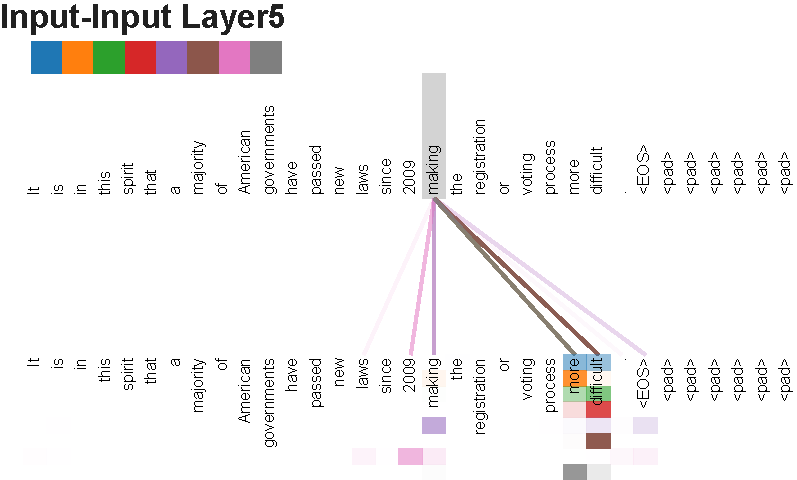
\includegraphics[width=\textwidth, trim=0 0 0 36, clip]{./vis/making_more_difficult5_new.pdf}}
\caption{一个展示编码器自注意力机制(第 5 层,共 6 层)中长距离依赖关系的注意力示例。许多注意力头关注动词 "making" 的远距离依赖,完成了短语 "making...more difficult"。此处仅展示单词 "making" 的注意力。不同颜色代表不同的注意力头。建议彩色查看。}
\end{figure*}

\begin{figure*}
{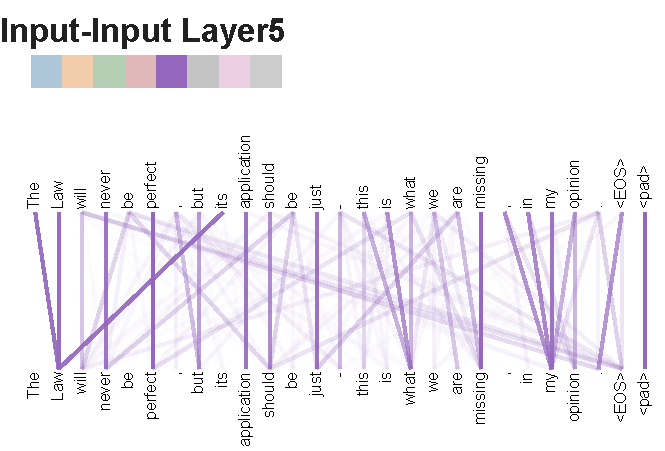
\includegraphics[width=\textwidth, trim=0 0 0 45, clip]{./vis/anaphora_resolution_new.pdf}}
{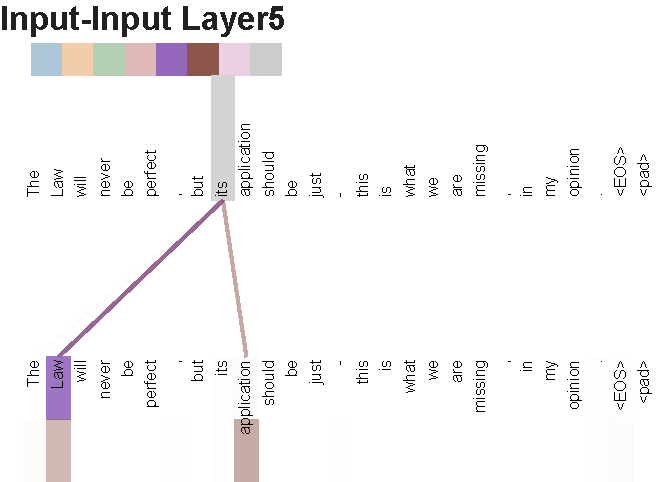
\includegraphics[width=\textwidth, trim=0 0 0 37, clip]{./vis/anaphora_resolution2_new.pdf}}
\caption{同样位于第 5 层(共 6 层)的两个注意力头,明显参与了 anaphora resolution(指代消解)。上图:头 5 的完整注意力。下图:仅针对单词 "its" 在头 5 和头 6 上的注意力隔离视图。注意该词的注意力分布非常集中。}
\end{figure*}

\begin{figure*}
{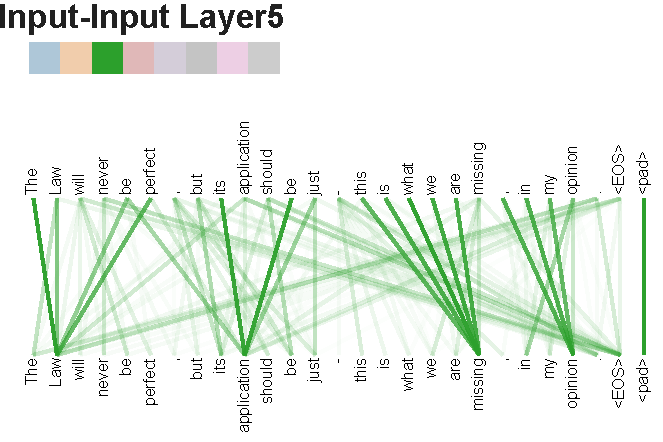
\includegraphics[width=\textwidth, trim=0 0 0 36, clip]{./vis/attending_to_head_new.pdf}}
{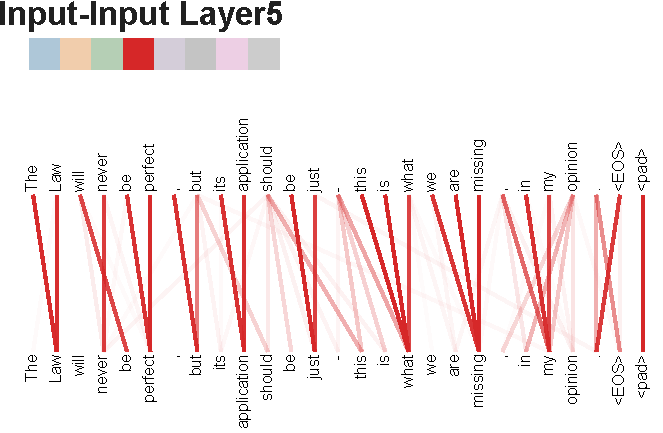
\includegraphics[width=\textwidth, trim=0 0 0 36, clip]{./vis/attending_to_head2_new.pdf}}
\caption{许多注意力头表现出与句子结构相关的行为模式。我们展示了来自编码器自注意力第 5 层(共 6 层)的两个不同头的两个此类示例。这些注意力头明显学会了执行不同的任务。}
\end{figure*}
